\subsection{Candidate Technologies}
Traditionally, edge devices were isolated gateways mainly forwarding traffic from their slaves to the cloud. This meant, all processing and storing was done in the cloud. Thus, the software of the gateways didn't need much management or maintenance. With advent of increased processing and storage at the edge, so called fog computing, the software on the gateways expanded to include business logic as well as routing. Today, gateways can be an integral part of the data flow, pre-processing data, filtering and storing data. However, this new software needs much more maintenance and management because changes in the business logic, e.g. API changes, need to be implemented in the gateway as well as on all other connected devices. With the advent of IIoT, the number of IoT gateways is set to increase dramatically and thus a solution for this problem has to be found.\\ This chapter will compare three different solutions for IoT gateways: Traditional gateway solutions, smart gateway solutions and gateways running on Kubernetes. First, a short overview of traditional gateway solutions is provided. Then, smart gateway solutions are defined and the Bosch IoT suite based on the OSGi technology is analyzed. Finally, gateway solutions based on kubernetes are presented and analyzed. The destinction between smart gateways and kubernetes based gateways is purely driven by kubernetes. It is the de-facto standard for cloud orchestration, has the support of (almost) all big IT companies and has many advantages over not so highly orchestration technologies.



The academic literature is not yet uniform in how to categorize IoT technolog

Open field --> work in progress so categories are not one implementation fits it all.

How should security be implemented.
Look into container and kubernetes security for IoT

How to solve low processing power of esp32?


provide many of the features cloud native (with containerization) do. Orchestrated solutions on the other hand offer a central configuration point, so a shared control plane between multiple gateways. These solutions were specifically developed for a distributed and large scale IoT environemnt. In many ways they are comparable to the solutions described in the next two subchapters, but are not developed with containerization at its foundation.

% https://scholar.google.com/scholar?cluster=13680069378267225814&hl=de&as_sdt=0,5
https://www.pac-online.com/sites/pac-online.com/files/upload_path/PDFs/Thema_des_Monats_Juni_2017_IoT_Plattformen.pdf
https://blog.bosch-si.com/bosch-iot-suite/lessons-learned-using-kubernetes-in-iot-deployments/

\subsection{Categorization of Gateways.}


\subsection{Traditional Gateway Solutions}
Tradition gateway solutions are all solutions which do not interact with data or only in a very limitted way and usually not content based. They are thus mainly forwarding data, i.e. operating as L3 device. The software running these devices is usually pre-installed by an OEM and hard to update and maintain. The gateways are isolated and information is only accumulated and processed in the cloud. Multiple gateways do not have a shared or centralized control plane and thus need to be managed independently and locally.\\
As these devices are still widely popular, they will form the base or reference case for this analysis. Compared to the next solutions, technologies in this category are not considered to do fog computing.


\subsection{Smart Gateway Solutions}
https://www.bosch-iot-suite.com/service/gateway-software/
Smart gateway solutions are all solutions which interact with their data on a business level perspective.

Smart gateway def  quotes:

[13] Internet of Things with Cloud Computing and the Issues Involved”, in
the proceedings of 11th IEEE International Bhurban Conference on
Applied Sciences and Technology, Islamabad, Pakistan, 14-18 January,
2014.
[14] Mohammad Aazam, Eui-Nam Huh, “Smart Gateway Based
Communication for Cloud of Things”, in the proceedings of 9th IEEE
International Conference on Intelligent Sensors, Sensor Networks, and
Information Processing, Singapore, 21-24 April, 2014.


But, they do not employ any cloud technologies like containers or kubernetes, even though the design philosophies are often overlapping. They may have a fully centralized configuration and control plane offering a central configuration point for multiple gateways or only parts of it. They may also take advantage of isolation to abstract in some form the underlying hardware.\\
The OSGi technology\cite{osgiDefintion25:online} is a aliance driven project from the Open Services Gateway initiative. It is a set of specifications (with reference implemetation and tests) for a dynamic modular system based on so called bundles, third party software, running on the Java Virtual Machine (JVM)\footnote{This means it is possible to use other languages apart from Java which can run in a JVM, e.g. Kotlin or Scala.}. The solution consists of a layered model shown in \cref{fig:osgiLayerModel}. 
\begin{figure}[h!]
    \centering
    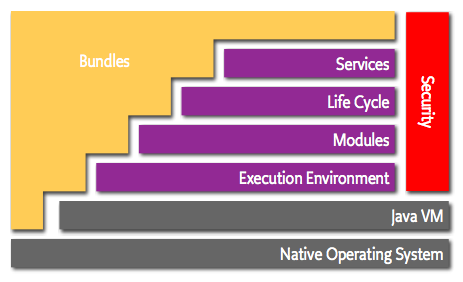
\includegraphics[scale=0.8]{figures/layering-osgi.png}
    \caption{From the official OSGI documentation\cite{osgiFrameworkArchitec22:online}.}
    \label{fig:osgiLayerModel}
\end{figure}
The Service layer interconnects the bundles making it possible for them to communicate via plain old java objects (POJO).The Life-Cycle layer handles the the state of the application (start, stop, update and uninstall). The Modules layer defines how an application can import and export code and the Execution Environemnt defines which methods and classes are available in a specific environemnt. Finally, the Security layer encompases all other layers and handles for example code authentication, the digital signing of jar files, file access restrictions, certificates and more.\\
There are currently six frameworks implementing the OSGi model which are under active development\footnote{This is to the authors best knowledge. Active development means, that security updates are still provided.}. One such solution is the Bosch IoT Gateway Software\cite{BoschIoT13:online}. In a blog entry from 2015 Bosch compares the OSGi technology to other gateway solutions and says it "is the only one with clearly defined specs and an open specification process behind them"\cite{boschBlogOSGi69:online}. Boschs solution is proprietary and tailer made for edge-computing devices with IIoT in mind\cite{OSGiforIoTBlog27:online}. It runs on Linux, Windows, mac OS, Android, and VxWorks and according to Bosch more than 40 different gateway devices\cite{BoschIoT13:online}. The software is stable at major version 9 and still under heavy development. Because of these reasons, it is used as an examplary solution. \Cref{fig:boschIoTGatewaySetup} shows where Boschs IoT solution is situated in the IoT environment. Bosch provides the OSGi framework implementation for the gateways and additional features for the cloud to ease the management of the gateways and store the accumulated data.
\begin{figure}[h!]
    \centering
    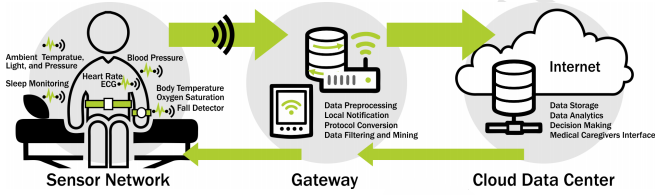
\includegraphics[scale=0.8]{figures/iotSetup.png}
    \caption{From the official Bosch documentation \cite{BoschIoT13:online}.}
    \label{fig:boschIoTGatewaySetup}
\end{figure}
A strong argument for this solution is the number of protocols it supports (BLE, ZigBee and MQTT, just to name a few) as well as its maturity.




\subsection{Containerized Gateway Solutions}

IoT cluster solutions\\
Isolated k8s cluster: Solution k3s\\
Kubernetes cluster where edge is part of the cloud: kubeedge\\
% https://github.com/kubernetes/website/pull/13158



\subsection{Cloud Native Gateway Solutions}
Edged: an agent that runs on edge nodes and manages containerized applications.
EdgeHub: a web socket client responsible for interacting with Cloud Service for the edge computing (like Edge Controller as in the KubeEdge Architecture). This includes syncing cloud-side resource updates to the edge, and reporting edge-side host and device status changes to the cloud.
CloudHub: a web socket server responsible for watching changes at the cloud side, caching and sending messages to EdgeHub.
EdgeController: an extended kubernetes controller which manages edge nodes and pods metadata so that the data can be targeted to a specific edge node.
EventBus: a MQTT client to interact with MQTT servers (mosquitto), offering publish and subscribe capabilities to other components.
ServiceBus: a HTTP client to interact with HTTP servers (REST), offering HTTP client capabilities to components of cloud to reach HTTP servers running at edge.
DeviceTwin: responsible for storing device status and syncing device status to the cloud. It also provides query interfaces for applications.
MetaManager: the message processor between edged and edgehub. It is also responsible for storing/retrieving metadata to/from a lightweight database (SQLite).

https://randomnerdtutorials.com/esp32-over-the-air-ota-programming/

file:///home/joe/Downloads/DDoS%20in%20the%20IoT%20Mirai%20and%20Other%20Botnets.pdf
Security containers:
Mirai attack: weak passwords, needs shell
Counter: Docker, binary files, non root user, 
traffic analysis via istio